\subsection{Modelo final}

Tras una fase intensiva de desarrollo e implementación de modelos generativos propios como GAN, cGAN y AttnGAN, se identificaron varias limitaciones que obstaculizaban el objetivo principal del proyecto: obtener imágenes visualmente coherentes y de calidad a partir de descripciones textuales. Entre los principales desafíos se encontraron la baja fidelidad visual de las imágenes generadas, la inestabilidad durante el entrenamiento y la elevada demanda de recursos computacionales. Ante este escenario, se optó por adoptar un enfoque basado en modelos preentrenados de alta calidad, siendo \textit{Stable Diffusion v1.4} el seleccionado por su equilibrio entre rendimiento, accesibilidad y resultados visuales.

\subsubsection{Motivación para el uso de modelos preentrenados}
El uso de modelos desarrollados desde cero permitió adquirir una comprensión profunda sobre los mecanismos de generación de imágenes, los procesos de codificación semántica del texto y el funcionamiento interno de arquitecturas como UNet o LSTM. Sin embargo, los resultados obtenidos no alcanzaban el nivel de calidad deseado, especialmente al trabajar con descripciones complejas del dataset COCO. Además, las restricciones computacionales (limitación de GPU, RAM y tiempo de entrenamiento) impedían escalar las pruebas de manera eficaz. Por ello, se decidió migrar a un modelo preentrenado que ofreciera resultados competitivos desde el inicio sin necesidad de un proceso de entrenamiento completo, siendo Stable Diffusion una de las soluciones más robustas disponibles actualmente para la generación de imágenes a partir de texto.

\subsubsection{Descripción del modelo: Stable Diffusion}
Stable Diffusion es un modelo generativo de código abierto basado en el paradigma de \textit{modelos de difusión latente}. A diferencia de los enfoques GAN, donde dos redes adversarias compiten entre sí, este modelo transforma una distribución de ruido gaussiano hacia una imagen coherente mediante un proceso de denoising progresivo. Todo el proceso se ejecuta dentro de un espacio latente comprimido, lo cual mejora considerablemente la eficiencia computacional sin sacrificar calidad visual.

\paragraph{\textbf{Componentes funcionales del modelo}} \mbox{}\\[0.5em]
El modelo se compone de varios módulos interconectados que trabajan en conjunto para transformar texto en imágenes. A continuación se presenta un resumen de los componentes principales y sus funciones:
\begin{table}[H]
\centering
\renewcommand{\arraystretch}{1.5}
\begin{tabular}{p{4.5cm}p{11cm}}
\rowcolor{gray!30}
\textbf{Componente} & \textbf{Función principal} \\
\rowcolor{gray!10}
\textbf{UNet2DConditionModel} & Red convolucional profunda que refina la imagen ruidosa en múltiples pasos, guiada por el texto. Se encarga del proceso de denoising en el espacio latente. \\
\textbf{CLIPTextModel (ViT-L/14)} & Codificador textual que convierte la descripción de entrada en una representación semántica densa utilizada como guía para el proceso de generación. \\
\rowcolor{gray!10}
\textbf{AutoencoderKL (VAE)} & Encargado de mapear imágenes reales al espacio latente y decodificar las imágenes generadas desde dicho espacio a píxeles reales. \\
\textbf{Scheduler (DDIM)} & Controla el ruido en cada paso y define la trayectoria de desdenoising, determinando el número de pasos y el ritmo de evolución. \\
\end{tabular}
\caption{Resumen funcional de los componentes principales de Stable Diffusion}
\label{tab:sd-components}
\end{table}

\paragraph{\textbf{Parámetros técnicos}} \mbox{}\\[0.5em]
Stable Diffusion v1.4 se caracteriza por una serie de parámetros técnicos que definen su arquitectura y funcionamiento. Estos parámetros son cruciales para entender el rendimiento del modelo y su capacidad de generar imágenes de alta calidad a partir de descripciones textuales. A continuación se detallan los más relevantes:
\begin{itemize}
\item \textbf{Resolución de entrada:} 512x512 píxeles.
\item \textbf{Tamaño del espacio latente:} 64x64 píxeles.
\item \textbf{Pasos de inferencia:} 50 (utilizando el scheduler DDIM).
\item \textbf{Guidance scale (CFG):} 7.5, valor que controla el grado de alineamiento entre texto e imagen.
\item \textbf{Codificador textual:} CLIP ViT-L/14.
\item \textbf{Parámetros de UNet:} Aproximadamente 860 millones.
\end{itemize}

\subsubsection{Evaluación inicial del modelo}

Como prueba exploratoria se utilizó el siguiente prompt genérico:

\begin{center}
\textit{``A beautiful landscape with mountains and a river''}
\end{center}

La imagen generada (Figura \ref{fig:original_image}) reflejó una notable fidelidad visual y semántica con respecto al texto, validando la capacidad del modelo para interpretar y representar con precisión elementos geográficos y naturales. Se observaron detalles como la correcta proporción entre los elementos, una distribución armónica del paisaje y un estilo visual coherente con la descripción dada.

Este resultado preliminar puso de manifiesto la solidez del modelo en tareas de generación generalista, especialmente con prompts descriptivos de carácter amplio. Asimismo, sirvió como punto de partida para contrastar su rendimiento en escenarios más exigentes o especializados, como la generación de razas de perros o conceptos personalizados que requieren una mayor precisión semántica.

\begin{figure}[H]
\centering
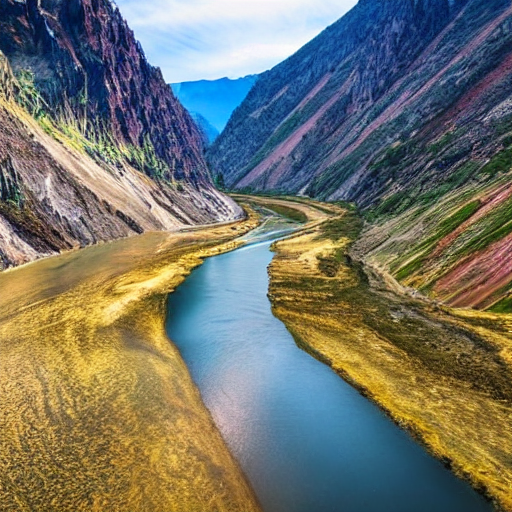
\includegraphics[width=0.4\textwidth]{original_output_image.png}
\caption{Imagen generada con Stable Diffusion v1.4 a partir del prompt \textit{``A beautiful landscape with mountains and a river''}.}
\label{fig:original_image}
\end{figure}

\subsubsection{Exploración de técnicas de optimización}
Pese a los buenos resultados iniciales, se evaluaron diversas estrategias para personalizar o mejorar el rendimiento del modelo. Estas técnicas permiten adaptar el modelo a tareas específicas, aumentar su capacidad expresiva o mejorar la coherencia semántica de las imágenes generadas con respecto al texto de entrada. A continuación se describen las principales aproximaciones consideradas:

\begin{itemize}
\item \textbf{Fine-tuning del modelo completo:} Ajuste de todos los pesos del modelo utilizando nuevos datos específicos. Esta técnica permite una especialización profunda, aunque conlleva un alto coste computacional y riesgo de sobreajuste si el conjunto de datos es reducido.

\item \textbf{Modificación del espacio latente:} Rediseño o ajuste del espacio latente en el que se realiza la generación, con el fin de mejorar la calidad representacional. Al trabajar en una representación comprimida, pequeñas mejoras en este espacio pueden traducirse en cambios significativos en la calidad y coherencia de las imágenes generadas.

\item \textbf{Reemplazo del VAE:} Sustitución del autoencoder variacional por uno más avanzado o con mejores propiedades de reconstrucción, lo cual puede influir positivamente en el nivel de detalle de las imágenes y reducir artefactos visuales en la salida final.

\item \textbf{Técnica LoRA:} (Low-Rank Adaptation) Permite modificar solo un subconjunto reducido de los parámetros del modelo mediante descomposición de matrices. Esto hace posible una adaptación eficiente con muy pocos recursos, sin necesidad de reentrenar el modelo completo.

\item \textbf{Cambio de función de pérdida:} Implementación de nuevas funciones de coste que optimicen no solo la precisión pixel a pixel, sino también la coherencia semántica o perceptual. Se pueden emplear pérdidas basadas en embeddings de CLIP o en distancias perceptuales como LPIPS.

\item \textbf{Modificaciones estructurales en UNet:} Inclusión de capas de atención adicionales (como Self-Attention o Cross-Attention), ajuste del número de bloques residuales o cambios en la arquitectura general. Estas modificaciones pueden aumentar la capacidad del modelo para capturar dependencias espaciales complejas.
\end{itemize}

Cada una de estas técnicas fue evaluada en términos de complejidad, coste computacional y mejora esperada en la calidad de las imágenes generadas. Se priorizó la búsqueda de un enfoque que permitiera una especialización rápida y efectiva sin requerir un reentrenamiento exhaustivo del modelo completo.

\subsubsection{Optimización seleccionada: modificación del espacio latente}
Tras comparar las distintas técnicas, se optó por modificar el espacio latente utilizando un enfoque inspirado en DreamBooth, que permite introducir nuevas clases visuales en el modelo sin reentrenar su totalidad. Esta técnica se basa en un entrenamiento ligero y dirigido, en el que el modelo aprende a asociar un término inventado con un concepto visual específico.

\paragraph{\textbf{Configuración del proceso}} \mbox{}\\[0.5em]
Para llevar a cabo la especialización del modelo, se utilizó el siguiente conjunto de parámetros y configuraciones:
\begin{itemize}
\item \textbf{Datos:} 60 imágenes de perros del dataset Stanford Dogs.
\item \textbf{Prompt condicional:} \texttt{``a photo of a sks dog''}.
\item \textbf{Entrenamiento:}
\begin{itemize}
\item Congelación de \texttt{CLIPTextModel} y \texttt{AutoencoderKL}.
\item Entrenamiento solo de \texttt{UNet2DConditionModel}.
\item Optimización con AdamW, batch size 1, learning rate $5\times10^{-6}$.
\item 1000 pasos de entrenamiento.
\end{itemize}
\end{itemize}

\paragraph{\textbf{Resultados}} \mbox{}\\[0.5em]
El proceso de especialización del modelo se completó en aproximadamente 5 horas, utilizando un servidor con dos GPUs NVIDIA TITAN RTX. El modelo resultante mostró una notable mejora en la generación de imágenes de perros: las imágenes generadas reflejaban con alta precisión los rasgos morfológicos de cada raza, se mantuvo la coherencia semántica con los nuevos \textit{prompts} específicos, y el entrenamiento resultó eficiente en tiempo y recursos, siendo compatible con entornos como Kaggle o servidores personales con GPU.

Como se ilustra en la Figura \ref{fig:latent-space-optimization}, el modelo es capaz de generar imágenes realistas y coherentes a partir de descripciones detalladas, como el prompt \textit{``a photo of a golden retriever wearing sunglasses''}, capturando tanto la raza como los elementos distintivos mencionados en el texto.

\begin{figure}[H]
\centering
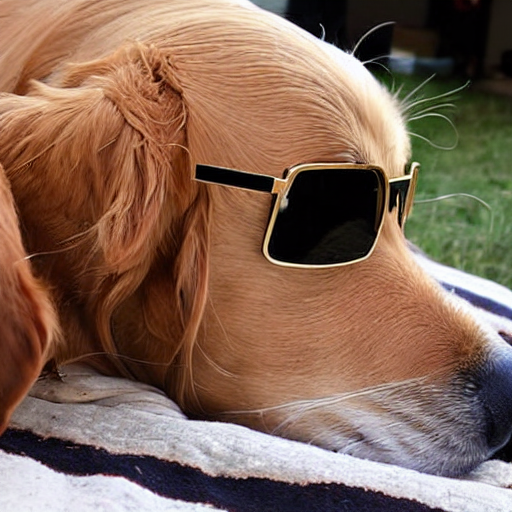
\includegraphics[width=0.45\textwidth]{golden_retriever.png}
\hfill
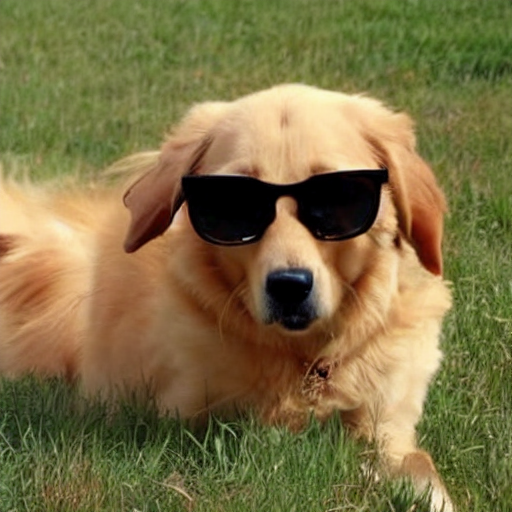
\includegraphics[width=0.45\textwidth]{golden_retriever-2.png}
\caption{Ejemplos de imágenes generadas tras la especialización del modelo con el prompt \textit{``a photo of a golden retriever wearing sunglasses''}.}
\label{fig:latent-space-optimization}
\end{figure}

\subsection{Evaluación y resultados}

Para validar la efectividad del proceso de especialización, se llevó a cabo una evaluación comparativa entre el modelo preentrenado y el modelo ajustado. Esta evaluación se centró en tres aspectos clave: fidelidad visual, coherencia semántica y adecuación morfológica a partir de un mismo prompt textual.

\subsubsection{Limitaciones del modelo base}

Aunque el modelo preentrenado Stable Diffusion v1.4 proporciona resultados visuales aceptables en muchos casos, se observaron importantes deficiencias al generar imágenes de conceptos específicos poco frecuentes, como ciertas razas de perros. Estas limitaciones afectan principalmente la coherencia anatómica y el realismo visual, lo que compromete su aplicabilidad en contextos especializados.

A modo de ejemplo, se utilizó el prompt:

\begin{center}
\textit{``a photo of a golden retriever''}
\end{center}

\subsubsection{Resultado con el modelo preentrenado}

La imagen generada por el modelo base presenta notables defectos: desalineación de los ojos, artefactos digitales en el hocico y una postura general poco natural. Aunque el color del pelaje podría sugerir la raza objetivo, la representación morfológica no es fiel ni reconocible.

\begin{figure}[H]
    \centering
    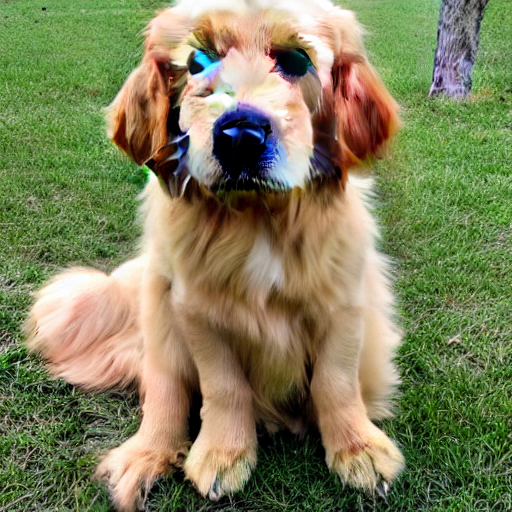
\includegraphics[width=0.45\textwidth]{golden_retriever_before.png}
    \caption{Resultado generado por el modelo preentrenado.}
    \label{fig:golden-before}
\end{figure}

\subsubsection{Resultado tras la especialización del modelo}

Tras aplicar la técnica de modificación del espacio latente, el modelo fue capaz de representar de forma mucho más precisa la raza solicitada. La imagen resultante muestra un perro con expresión realista, pelaje detallado, proporciones correctas y una pose reconocible. El resultado evidencia una mejora tanto estética como semántica.

\begin{figure}[H]
    \centering
    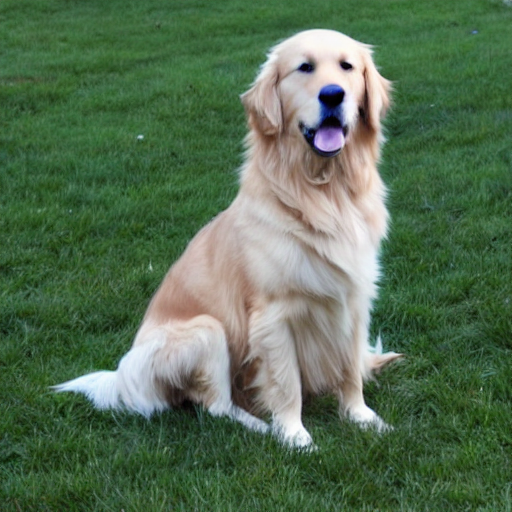
\includegraphics[width=0.45\textwidth]{golden_retriever_after.png}
    \caption{Resultado generado tras la especialización del modelo.}
    \label{fig:golden-after}
\end{figure}

\subsubsection{Evaluación de coherencia semántica con CLIP}

Para respaldar cuantitativamente esta mejora, se empleó el modelo \texttt{CLIP ViT-L/14}, que permite calcular la similitud entre imágenes y texto. Se utilizó el concepto de \textit{CLIP Score relativo}, que compara la afinidad de dos imágenes frente a un mismo prompt.

\begin{table}[H]
\centering
\renewcommand{\arraystretch}{1.5}
\begin{tabular}{|p{6cm}|c|}
\hline
\rowcolor{gray!30}
\textbf{Imagen generada} & \textbf{CLIP Score relativo} \\
\hline
Modelo preentrenado & 0.0659 \\
\hline
Modelo especializado & 0.9341 \\
\hline
\end{tabular}
\caption{Similitud relativa medida con CLIP}
\label{tab:clip-golden}
\end{table}

\begin{figure}[H]
    \centering
    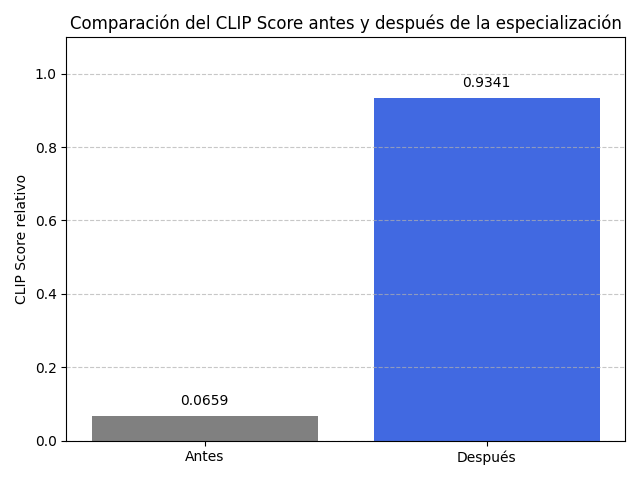
\includegraphics[width=0.45\textwidth]{clip-bar.png}
    \caption{Comparación visual del CLIP Score relativo.}
    \label{fig:clip-bar}
\end{figure}

\subsubsection{Síntesis de resultados}

La Figura~\ref{fig:clip-bar} visualiza de forma clara la mejora lograda. Mientras que el modelo original apenas logra asociar la imagen con el concepto de “golden retriever”, el modelo especializado alcanza un nivel de coherencia semántica casi perfecto. Esto confirma que la técnica utilizada no solo mejora la calidad visual, sino también la capacidad del modelo para representar correctamente conceptos específicos.

\subsubsection{Análisis del coste de entrenamiento}

Para evaluar la viabilidad del entrenamiento personalizado, se midieron los principales factores que impactan en el coste computacional del proceso. Estos valores permiten estimar la escalabilidad del enfoque en distintos entornos de ejecución.

\begin{table}[H]
\centering
\renewcommand{\arraystretch}{1.5}
\begin{tabular}{|p{5cm}|p{9cm}|}
\hline
\rowcolor{gray!30}
\textbf{Recurso} & \textbf{Especificaciones del servidor utilizado} \\
\hline
Procesador & AMD Ryzen Threadripper 2920X, 12 núcleos físicos, 24 hilos, hasta 3.5 GHz \\
\hline
Memoria RAM & 62 GiB totales, disponibles: 60 GiB libres \\
\hline
GPU & 2x NVIDIA TITAN RTX, 24 GiB de VRAM cada una \\
\hline
Sistema operativo & Ubuntu 24.04, kernel 6.8.0-59-generic, arquitectura x86\_64 \\
\hline
CUDA y Drivers & CUDA 12.4, Driver NVIDIA 550.163.01 \\
\hline
Duración del entrenamiento & Aprox. 5 horas \\
\hline
Tamaño del modelo entrenado & 4.0K (tamaño en disco del directorio \texttt{stable-dog-output}) \\
\hline
Frameworks utilizados & \texttt{diffusers}, \texttt{transformers}, \texttt{PyTorch}, \texttt{torchvision} \\
\hline
Técnicas aplicadas & DreamBooth, checkpointing, half precision (float16), batch size adaptativo \\
\hline
\end{tabular}
\caption{Recursos técnicos del servidor utilizado para el entrenamiento final}
\label{tab:servidor-entrenamiento}
\end{table}

\subsubsection{Evaluación de la generalización del modelo}

Además de mejorar la generación de razas específicas como el \textit{golden retriever}, resulta clave comprobar si el modelo especializado conserva su capacidad para generar imágenes no relacionadas con el entrenamiento. Para ello, se utilizó un prompt genérico:

\begin{center}
\textit{``a man sitting on a bench in a park''}
\end{center}

La generación se realizó antes y después de aplicar la especificación para evaluar posibles pérdidas de generalidad.

\paragraph{\textbf{Antes del entrenamiento especializado}} \mbox{}\\[0.5em]
El modelo preentrenado genera una escena coherente: un hombre de espaldas sentado en un banco, con árboles bien definidos y composición equilibrada. El resultado es visualmente aceptable y semánticamente correcto.

\begin{figure}[H]
    \centering
    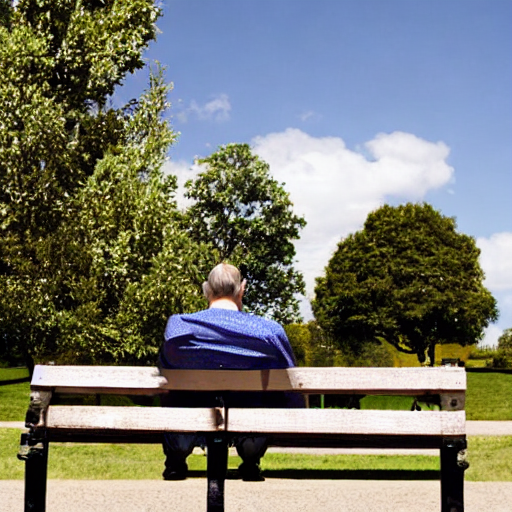
\includegraphics[width=0.45\textwidth]{man_before.png}
    \caption{Imagen generada por el modelo base con el prompt ``a man sitting on a bench in a park''.}
    \label{fig:man-before}
\end{figure}

\paragraph{\textbf{Después del entrenamiento especializado}} \mbox{}\\[0.5em]
Tras la especialización en razas de perro, el modelo mantiene su capacidad para representar correctamente conceptos no entrenados. La escena generada presenta un entorno similar, con árboles, banco y persona reconocibles, sin signos de sobreajuste. Esto sugiere que la adaptación ha sido localizada y no ha afectado negativamente a la generalización.

\begin{figure}[H]
    \centering
    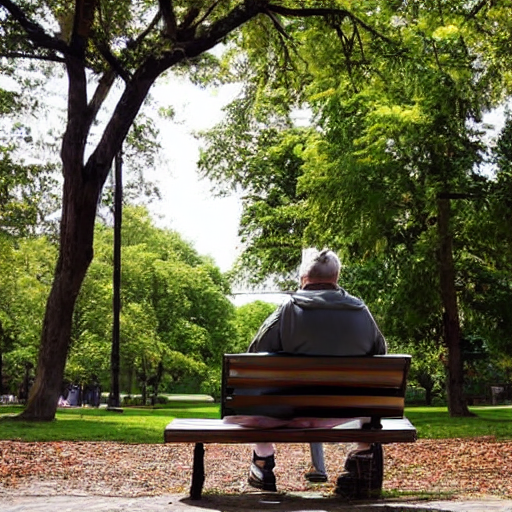
\includegraphics[width=0.45\textwidth]{man_after.png}
    \caption{Imagen generada por el modelo especializado con el mismo prompt.}
    \label{fig:man-after}
\end{figure}

\paragraph{\textbf{Conclusión}} \mbox{}\\[0.5em]
La comparación cualitativa sugiere que el modelo mantiene una buena capacidad de generalización tras la especialización. Es capaz de generar imágenes coherentes incluso para descripciones no incluidas en el entrenamiento, lo que refuerza la aplicabilidad del enfoque de DreamBooth en contextos donde es crucial preservar el conocimiento base del modelo.
